%!TEX program = xelatex
% 完整编译方法 1 pdflatex -> bibtex -> pdflatex -> pdflatex
% 完整编译方法 2: xelatex -> bibtex -> xelatex -> xelatex
\documentclass[lang=cn,11pt]{elegantpaper}

\title{基于Hadoop MapReduce并行计算框架的邮件自动分类}
\author{曹佳涵 $\quad$ 白家杨 $\quad$ 刘笑今}

\institute{2019st04小组}

% 不需要版本信息,直接注释即可
\version{}
% 不需要时间信息的话,需要把 \today 删除。
\date{}


% 如果想修改参考文献样式,请把这行注释掉
\usepackage[authoryear]{gbt7714}  % 国标

\begin{document}

\maketitle

\begin{abstract}
\noindent 本实验的目标是通过 MapReduce 编程来实现邮件的自动分类,通过本课程设计的学习,可以体会如何使用 MapReduce 完成一个综合性的数据挖掘任务,包括全流程的数据预处理、样本分类、样本预测等。我们使用Hadoop MapReduce并行计算框架对原始邮件文本进行特征选择、特征向量权重计算、文本分类和样本预测任务,从而搭建起一个完整的文本分类处理流程。我们采用了不同的特征提取方法和分类算法并进行比较和分析。此外,我们使用Spark同样完成了实验。
\keywords{邮件分类,并行计算,MapReduce,Spark}
\end{abstract}

\section{引入}



此模板是基于 \LaTeX{} 的标准文类 article设计,也即意味着你可以把 article 文类的选项传递给本模板,比如 \lstinline{a4paper, 10pt} 等等(推荐使用 \lstinline{11pt})。本模板支持 \lstinline{PDFLaTeX} 和 \lstinline{XeLaTeX}\footnote{中文字体均使用 \lstinline{ctex} 包设置。} 两种编译方式。

数学字体的效果如下:

\begin{equation}
(a+3b)^{n} = \sum_{k=0}^{n} C_{n}^{k} a^{n-k} (3b)^k\label{eq:binom}
\end{equation}
      
\subsection{全局选项}
我在这个模板中定义了一个语言选项 \lstinline{lang},可以选择英文模式 \lstinline{lang=en}(默认)或者中文模式 \lstinline{lang=cn}。当选择中文模式时,图表的标题引导词以及参考文献,定理引导词等信息会变成中文。你可以通过下面两种方式来选择语言模式:

\begin{lstlisting}
\documentclass[lang=cn]{elegantpaper} % or
\documentclass{cn}{elegantpaper} 
\end{lstlisting}


\subsection{自定义命令}
在此模板中,并没有修改任何默认的命令或者环境,所以,你可以在此模板使用原来的命令和环境。另外,我自定义了 3 个命令:

\begin{enumerate}
	\item \lstinline{\email}:创建邮箱地址的链接;
	\item \lstinline{\figref}:用法和 \lstinline{\ref} 类似,但是会在插图的标题前添加 <\textbf{图 n}> ;
	\item \lstinline{\tabref}:用法和 \lstinline{\ref} 类似,但是会在表格的标题前添加 <\textbf{表 n}>;
	\item \lstinline{\keywords}:为摘要环境添加关键词。
\end{enumerate}

\subsection{列表环境}
你可以使用列表环境(\lstinline{itemize}、\lstinline{enumerate}、\lstinline{description}),示例如下:\\[2ex]
\begin{minipage}[c]{0.59\linewidth}
\begin{lstlisting}
\begin{itemize}
   \item Routing and resource discovery;
   \item Resilient and scalable networks; 
   \item Distributed storage and search.
\end{itemize}
\end{lstlisting}
\end{minipage}
\begin{minipage}[c]{0.4\linewidth}
\begin{itemize}
   \item Routing and resource discovery;
   \item Resilient and scalable networks;
   \item Distributed storage and search.
\end{itemize}
\end{minipage}




\subsection{插图}
插图的命令和以前一样,也是使用 \lstinline{figure} 环境。\figref{fig:scatter} 显示了插图的效果。你可以把你的图放到当前工作目录的如下子目录下 (\lstinline{./image/}, \lstinline{./img/}, \lstinline{./figure/}, \lstinline{./fig/})。


\begin{lstlisting}
\begin{figure}[htbp]
	\centering
	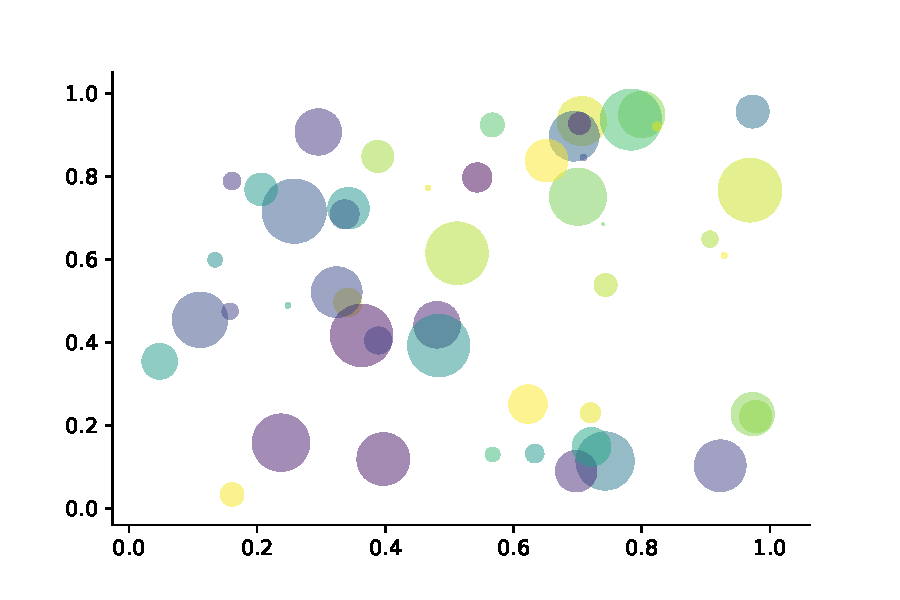
\includegraphics[width=0.6\textwidth]{scatter.pdf}
	\caption{Scatter Plot Example \label{fig:scatter}}
\end{figure}
\end{lstlisting}
\begin{figure}[htbp]
	\centering
	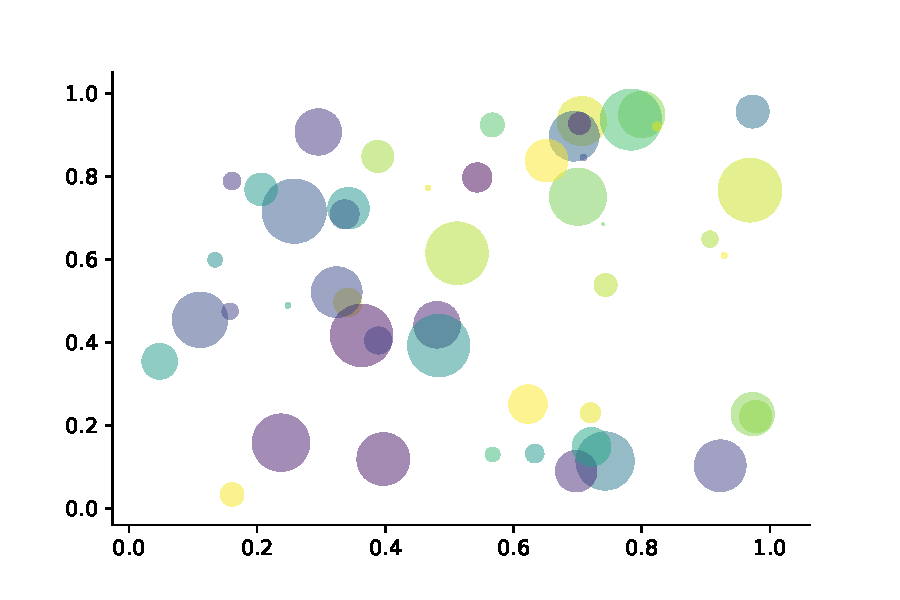
\includegraphics[width=0.6\textwidth]{scatter.pdf}
	\caption{Scatter Plot Example \label{fig:scatter}}
\end{figure}

\subsection{表格}
我强烈建议你使用 \lstinline{booktabs} 宏包,这个宏包有三个命令 \lstinline{\toprule}、\lstinline{\midrule} 和 \lstinline{\bottomrule} 能方便你制作三线表。\tabref{tab:reg} 是一个示例:

\begin{lstlisting}
\begin{table}[htbp]
  \small
  \centering
  \caption{Auto MPG and Price \label{tab:reg}}
    \begin{tabular}{lcc}
    \toprule
                    &       (1)         &        (2)      \\
    \midrule
    mpg             &    -238.90***     &      -49.51     \\
                    &     (53.08)       &      (86.16)    \\
    weight          &                   &      1.75***    \\
                    &                   &      (0.641)    \\
    constant        &     11,253***     &       1,946     \\
                    &     (1,171)       &      (3,597)    \\
    obs             &        74         &         74      \\
    $R^2$           &      0.220        &       0.293     \\
    \bottomrule
    \multicolumn{3}{l}{\scriptsize Standard errors in parentheses} \\
    \multicolumn{3}{l}{\scriptsize *** p<0.01, ** p<0.05, * p<0.1} \\
    \end{tabular}%
\end{table}%
\end{lstlisting}
\begin{table}[htbp]
  \small
  \centering
  \caption{Auto MPG and Price \label{tab:reg}}
    \begin{tabular}{lcc}
    \toprule
                    &       (1)         &        (2)      \\
    \midrule
    mpg             &    -238.90***     &      -49.51     \\
                    &     (53.08)       &      (86.16)    \\
    weight          &                   &      1.75***    \\
                    &                   &      (0.641)    \\
    constant        &     11,253***     &       1,946     \\
                    &     (1,171)       &      (3,597)   \\
    obs             &        74         &         74     \\
    $R^2$           &      0.220        &       0.293    \\
    \bottomrule
    \multicolumn{3}{l}{\scriptsize Standard errors in parentheses} \\
    \multicolumn{3}{l}{\scriptsize *** p<0.01, ** p<0.05, * p<0.1} \\
    \end{tabular}%
\end{table}%



\subsection{参考文献}
你可以在谷歌学术,Mendeley,Endnote 中获得文献条目(bib item),然后把它们添加到 \lstinline{wpref.bib} 中。在文中引用的时候,引用它们的键值(bib key)即可。注意需要在编译的过程中添加 Bib\TeX{} 编译。如果你想在参考文献中添加未引用的文献(部分或者全部),可以使用

\begin{lstlisting}
\nocite{EINAV2010, Havrylchyk2018} % add the two reference.
\nocite{*}   % add all the reference in the bib file.
\end{lstlisting}

如果你想修改参考文献的样式(比如改为 \lstinline{aer}),你可以在导言区将下面代码注释掉。
\begin{lstlisting}
\usepackage[authoryear]{gbt7714}
\end{lstlisting}

并且文档末尾添加

\begin{lstlisting}
\bibliographystyle{aer}
\end{lstlisting}

\section{数据分析}
对于训练数据,经过分析,共有20个类别,它们编号,名称,以及包含的邮件文本个数为:\par
\begin{table}[htbp]
  \small
  \centering
  \caption{Auto MPG and Price \label{tab:reg}}
    \begin{tabular}{lcc|lcc}
    \toprule
    类别编号  &   类别名称  &   包含邮件文本个数  &   类别编号  & 类别名称  & 包含邮件文本个数  \\
    \hline
    1 & sci.electronics & 1000            & 11 & rec.sport.baseball & 1000 \\
    2 & comp.windows.x & 1000             & 12 & rec.autos & 1000 \\
    3 & talk.politics.mideast & 1000      & 13 & talk.politics.misc & 1000 \\
    4 & comp.os.ms-windows.misc & 1000    & 14 & talk.politics.guns & 1000 \\
    5 & rec.sport.hockey & 1000           & 15 & comp.graphics & 1000 \\
    6 & sci.crypt & 1000                  & 16 & soc.religion.christian & 997 \\
    7 & comp.sys.mac.hardware & 1000      & 17 & rec.motorcycles & 1000 \\
    8 & sci.space & 1000                  & 18 & misc.forsale & 1000 \\
    9 & talk.religion.misc & 1000         & 19 & sci.med & 1000 \\
    10 & comp.sys.ibm.pc.hardware & 1000  & 20 & alt.atheism & 1000 \\
    \bottomrule
    \end{tabular}%
\end{table}%\
可以看到,训练样本全集共有20个类别,训练样本总数为19997个,每个类别下训练样本的数量是平衡的,几乎都是1000个,因此在进行训练时,不需要考虑类别不平衡问题。


\section{MapReduce处理流程}
\subsection{特征选择}
本任务的主要工作是对原始的邮件文本中进行特征选择,选择出能够表征邮件主题的特征词,为后续的文本分类做准备。\par
对于输入的未分词的邮件训练样本全集和停词表,我们需要输出全局邮件文本特征,并对它们进行相应的编号,此外,对于训练数据集的目录,将目录名(即文本类别)转换为相应的类别序号。\par
对于该步骤,我们采用了两种计算方法,分别为半并行化和并行化计算方法。
\subsubsection{半并行化计算方法}
半并行化计算方法是指将该任务划分为两个步骤,第一步读取训练样本全集和停词表,生成干净文本;第二步读取干净文本,生成全局邮件特征集。\par
第一步的主要思路是顺序执行,首先读取20\_newsgroup文件夹下的子文件夹,将子文件夹名(即类别名)转化为类编号并进行存储。将 Lucene 的 Standard Analyzer 分词器作为基类,输入停词表,自定义自己的带有停词表功能的停词器,然后顺序依次读取每个子文件夹下的所有文件,使用自定义的停词器对文本进行分词,并将分词结果储存在目标文件中,我们将分词后的文本称为干净文本,生成干净文本的过程是顺序执行,非并行化的。为了后续处理的方便性,我们修改输出文件的格式为:filename-classNum,filename为原文件的文件名,classNum为它所属的类别的编号,两者用分隔符 '-' 隔开。\par
伪代码如下:
\begin{algorithm}[htb]  
  \caption{特征选择半并行化算法:第一步}
  \label{alg:Framwork}
  \begin{algorithmic}[1]
    \Require
    邮件训练样本全集 $U$,停词表 $S$
    \Ensure
    用停词表分割后的干净文本
    \State 初始化类别名-类别编号对应表 classMap
    \State 初始化停词器 stopAnalyzer=StopAnalyzer($S$)
      \For{each 文本 $u$ in $U$}
      \State 新文本 $u^\prime$ = stopAnalyzer(u)
      \State 通过类别名-编号对应表查找文本$u$的文件名filename对应的类别编号num=classMap($u$)
      \State 在目标目录下创建filename-num文件,并将新文本$u^\prime$的内容写入该文件。
   \EndFor
  \end{algorithmic}
\end{algorithm}
第二步从干净文本中提取全局邮件文本特征集的过程是并行化的,使用MapReduce并行计算框架,在Map阶段读取干净文本,对于每一个单词word,发射(word,1)键值对。在Reduce阶段,设置一个全局缓存变量$n$,为每个单词维护一个编号,并将每个单词和相应的编号输出到全局邮件特征集中。\par
伪代码如下:
\begin{algorithm}[htb]
  \caption{特征选择半并行化算法:第二步}
  \label{alg:Framwork}
  \begin{algorithmic}[1]
    \Require
    干净文本 $U^\prime$
    \Ensure
    \State \textbf{Map阶段}:
    \Function {map}{$filename$, $text$}
      \For{each word $w$ in $text$}
        \State Emit($w$,$1$)
      \EndFor
    \EndFunction
    \State \textbf{Reduce阶段}:
    \Function {reduce}{$word$, $value$}
      \State 全局缓存变量$num=num+1$
      \State 将$word$和$num$写入到全局邮件文本特征集中
      \State Emit($word$,$value$)
    \EndFunction
  \end{algorithmic}
\end{algorithm}

\subsubsection{并行化计算方法}
非并行化顺序执行,缺点也显而易见:计算速度慢,效率低,因此我们设计了并行化的计算方法,利用 MapReduce 计算框架,很好地并行处理大量的训练文本,极大地加快了处理速度。\par
在Map阶段读取原文本,利用停词器将其分词后输出到目标目录下,同时对于每一个单词,发射(word,filename-classNum)键值对。值得注意的是,因为停词表是所有Mapper都需要各自初始化的,因此将其初始化放在Map阶段的setup过程中,首先将停词表文件路径存在DistributedCache中,然后在setup过程中读取该路径并利用其初始化停词器,在map过程中使用该停词器。\par
在Reduce阶段,设置一个全局缓存变量$n$,用来表示每一个单词的唯一标号。输入为(word, value)。由于在Reduce阶段,已经将相同key的键值对都整合到了一起,因此读取的word值是唯一不重复的,只需要利用全局变量$n$为每一个单词分配相应的标号,并将单词和编号输出到目标文件中即可。\par
伪代码如下:
\begin{algorithm}[htb]  
  \caption{特征选择并行化算法}  
  \label{alg:Framwork}
  \begin{algorithmic}[1]
    \Require
    邮件训练样本全集 $U$,停词表 $S$
    \Ensure 
    用停词表分割后的干净文本,全局邮件文本特征集
    \State 初始化类别名-类别编号对应表 classMap
    \State 将停词表$S$ 存入DistributedCache中
    \State \textbf{Map阶段}:
    \Function {setup}{}
    \State 从DistributedCache中读取停词表$S$
    \State 初始化停词器 stopAnalyzer=StopAnalyzer($S$)
    \EndFunction
    \Function {map}{$filename$, $text$}
      \State $text^\prime$ = stopAnalyzer($text$)
      \State 将$text^\prime$写入到目标干净文本中
      \For{each word $w$ in $text^\prime$}
        \State Emit($w$,$filename$)
      \EndFor
    \EndFunction
    \State \textbf{Reduce阶段}:
    \Function {reduce}{$word$, $value$}
      \State 全局缓存变量$num=num+1$
      \State 将$word$和$num$写入到全局邮件文本特征集中
      \State Emit($word$,$filename$)
    \EndFunction
  \end{algorithmic}
\end{algorithm}

\subsubsection{运行结果}
该任务的输出结果如下图所示:
\begin{figure}[htbp]
	\centering
	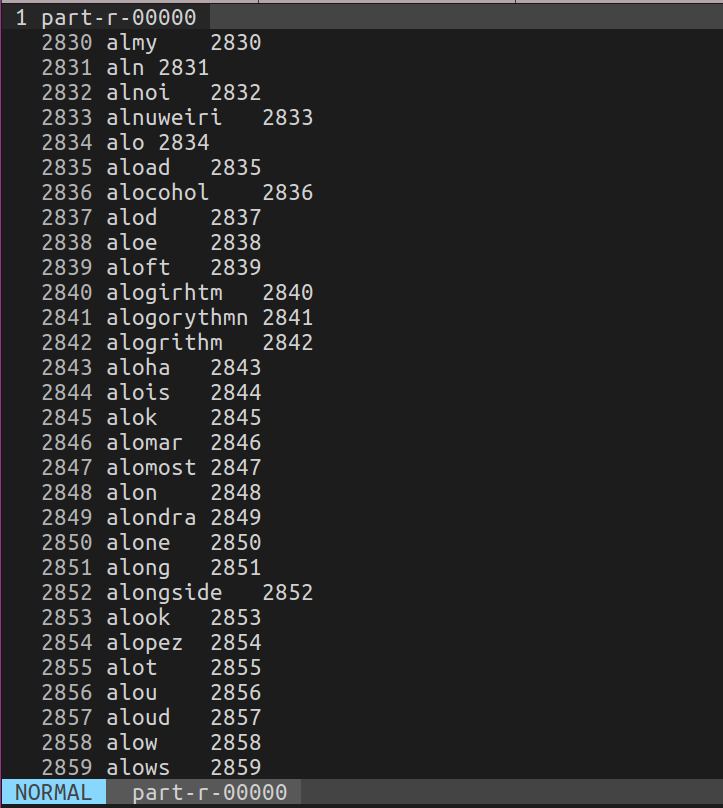
\includegraphics[width=0.6\textwidth]{feature-out.png}
	\caption{全局邮件文本特征 \label{fig:feature-out}}
\end{figure}

\subsection{朴素贝叶斯}
\subsubsection{原理推导}
朴素贝叶斯算法是生成模型中分类算法之一。所有朴素贝叶斯分类器都假设特定特征的值独立于给定类变量的任何其他特征的值。例如,如果水果是红色的,圆形的,直径约10厘米,则可以认为它是苹果。朴素贝叶斯分类器认为这些特征中的每一个都独立地贡献于该果实是苹果的概率,而不管任何可能的颜色,圆度和直径特征之间的相关性。

抽象来看,朴素贝叶斯是一个条件概率模型:给定一个要分类的问题实例,用向量表示 $ \mathbf {x} =(x_ {1} , \dots, x_ {n})$代表一些n个特征(自变量),它为这个实例分配概率$p(C_ {k} \mid x_ {1}, \dots, x_ {n})$其中$C_{k}$表示$K$个可能的类别中的一个 。

使用贝叶斯定理,条件概率可以分解为
$$
p(C_ {k} \mid \mathbf {x})= {\frac {p(C_ {k})p (\mathbf {x} \mid C_ {k})} {p(\mathbf {x} )}}
$$
“朴素”的条件独立假设发挥作用:假设所有特征都在$\mathbf {x}$是相互独立的,对类的条件$ C_ {k}$。在这个假设下,
$$
p(x_ {i}\mid x_ {i+1},\dots,x_ {n},C_ {k})= p(x_ {i} \mid C_ {k})
$$
因此,可以表示为
$$
p(C_ {k} \mid x_ {1},\dots,x_ {n})= \frac{p(C_ {k})}{p(\mathbf {x})}\prod_ {i = 1}^{n} p(x_ {i} \mid C_ {k})
$$
因此只要比较$p(C_ {k})\prod_ {i = 1}^{n} p(x_ {i} \mid C_ {k})$的值就可以判断类别。即为求下式
$$
\hat{y} = {\underset {k \in \ {1,\dots,K}} {\operatorname {argmax}}} \ p(C_ {k})\prod_{i = 1} ^ {n} p(x_ {i} \mid C_ {k})
$$
常用的有高斯朴素贝叶斯,伯努利朴素贝叶斯Bernoulli和多项式朴素贝叶斯Multinomial三种。

高斯朴素贝叶斯当处理连续数据时,典型的假设是与每个类相关联的连续值根据正态(或高斯)分布分布。

多项式朴素贝叶斯使用多项事件模型,样本(特征向量)表示多项式生成某些事件的频率 $(p_ {1},\dots,p_ {n})$其中 $p_i$是事件i发生的概率(或多类情况下的K个多项式)。在词袋模型中事件表示单个文档中单词的出现。

伯努利朴素贝叶斯:在多变量伯努利事件模型中,特征是描述输入的独立布尔值(二元变量)。

尽管朴素贝叶斯分类器具有朴素设计和明显过于简单的假设,但它在许多复杂的现实世界中仍然运行良好。综合比较表明,贝叶斯分类的表现优于其他方法,特别是在文本处理方面。

\subsubsection{hadoop实现}

词袋模型就是表示文本特征的一种方式。给定一篇文档,它会有很多特征,比如文档中每个单词出现的次数、某些单词出现的位置、单词的长度、单词出现的频率……而词袋模型只考虑一篇文档中单词出现的频率(次数),用每个单词出现的频率作为文档的特征(或者说用单词出现的频率来代表该文档)。利用词袋模型表示文本特征来进行朴素贝叶斯分类器的实现。

实际上就是求
$$
\hat{y} = {\underset {k \in \ {1,\dots,K}} {\operatorname {argmax}}} \ p(C_ {k})\prod_{i = 1} ^ {n} p(w_ {i} \mid C_ {k})
$$
其中$w_i$表示文档中的第i个单词。

由于每个概率值很小(比如0.0001)若干个很小的概率值直接相乘,得到的结果会越来越小。为了避免计算过程出现下溢,最终无法比较,引入对数函数Log,在 Log 空间中进行计算。然后得到如下公式
$$
\hat{y} = {\underset {k \in \ {1,\dots,K}} {\operatorname {argmax}}} \ log \ p(C_ {k}) + \sum_{i = 1} ^ {n} log \ p(w_ {i} \mid C_ {k})
$$
训练朴素贝叶斯的过程其实就是计算先验概率$p(C_k)​$和后半部分似然函数的过程。

\subsubsection{先验概率p(c)的计算}

$P(C_k)$的意思是:在所有的文档中,类别为$C_{k}$的文档出现的概率有多大。假设训练数据中一共有$N_{doc}$篇文档,只要数一下类别$C_{k}$的文档有多少个就能计算$P(C_k)$了,类别$C_{k}$的文档共有$N_k$篇,先验概率的计算公式如下:
$$
p(C_k)=\frac{N_K}{N_{doc}}
$$
\subsubsection{似然函数$p(w_i|C_k)$的计算}

由于是用词袋模型表示一篇文档d,对于文档d中的每个单词$w_i$,找到训练数据集中所有类别为$C_{k}$的文档,数一数 单词$w_i$在这些文档(类别为$C_{k}$)中出现的次数:$count(w_{i},C_{k})$。

然后,再数一数训练数据集中类别为$C_{k}​$的文档一共有多少个单词
$$
\sum_{w \in v}count(w, C_{k})
$$
其中V是词库,即所有在文本中出现过的单词。(有些单词在词库中,但是不属于类别$C_{k}$,那么 $count(w, C_{k}) = 0​$

计算二者之间的比值,就是似然函数的值。似然函数计算公式如下:
$$
p(w_ {i} \mid C_ {k})=\frac{count(w_i, C_k)}{\sum_{w \in v}count(w, C_{k})}
$$
需要考虑特殊情况某一类的文档不包含某个词时,考虑add-one-smoothing,类似于拉普拉斯修正,其实就是将“出现次数加一”。此时似然函数变为:
$$
p(w_ {i} \mid C_ {k})=\frac{count(w_i, C_k)+1}{\sum_{w \in v}(count(w, C_{k})+1)}=\frac{count(w_i, C_k)+1}{\sum_{w \in v}count(w, C_{k})+|V|}
$$
其中$|V|$表示词库的单词数。

在hadoop的实现中分成了两个Job来完成,分别是训练阶段的Job和预测阶段的Job
\begin{algorithm}[htb]
  \caption{朴素贝叶斯训练阶段第一个Job}
  \label{alg:Framwork}
  \begin{algorithmic}[1]
    \Require
    邮件训练样本全集 $U$
    \Ensure
    输出训练结果文件,记录键值对<类名\#单词,数量>
    \State Map阶段:分割每个单词并根据文件名获得类名编号,输出<类名\#单词,数量>
    \For{each 单词 $w$ in $U$}
      \State 类名编号$classnum = GetClassNum(GetFileName(w))$
      \State Emit($classnum + "\#" + w$, 1)
   \EndFor
	\State Combine阶段:合并<类名\#单词,num1>、<类名\#单词,num2>为<类名\#单词,num1+num2>
    \State Reduce阶段:合并并输出<类名\#单词,数量>到输出文件中
    \State sum = 0
	\For{all <类名\#单词,数量num> with same key}
      \State 类名编号$sum += num$

   \EndFor
	\State Emit(类名\#单词, sum)
  \end{algorithmic}
\end{algorithm}

\begin{algorithm}[htb]
  \caption{朴素贝叶斯预测阶段第二个Job}
  \label{alg:Framwork}
  \begin{algorithmic}[1]
    \Require
    第一个Job训练结果键值对集合$<>$训练邮件预测样本全集 $U$, 类编号和类文件数对应表$B$
    \Ensure
    输出训练结果文件,记录键值对<类名\#单词,数量>
    \State Map阶段:分割每个单词并根据文件名获得类名编号,输出<类名\#单词,数量>
	\State Map阶段setup:将训练结果$A$键值对保存到Map<String, int>结构的TrainSet中,并提取键值对<类名\#单词,数量>中的单词存入词库WordSum中
	\State Map阶段setup:将对应关系$B$保存到Map<String, int>结构的ClassSet中
	\State Map阶段map:
    \For{each 单词 $w$ in $U$}
      \State 类名编号$classnum = GetClassNum(GetFileName(w))$
		\For{each 类别 $c$ in ClassSet.keys}
      		\State 类名编号$classnum = GetClassNum(GetFileName(w))$
      		\State Emit($classnum + "\#" + w$, 1)
   			\EndFor
      \State Emit($classnum + "\#" + w$, 1)
   \EndFor
	\State Combine阶段:合并<类名\#单词,num1>、<类名\#单词,num2>为<类名\#单词,num1+num2>
    \State Reduce阶段:合并并输出<类名\#单词,数量>到输出文件中
    \State sum = 0
	\For{all <类名\#单词,数量num> with same key}
      \State 类名编号$sum += num$

   \EndFor
	\State Emit(类名\#单词, sum)
  \end{algorithmic}
\end{algorithm}



\end{document}
